\documentclass{beamer}
\usepackage{graphicx}
\usepackage[most]{tcolorbox}
\usepackage{xcolor}
\definecolor{lightblue}{RGB}{25, 25, 112} % RGB-Werte für Hellblau

\usetheme{CambridgeUS}
\usecolortheme{dolphin}

\title{Verteilte Systeme}
\subtitle{Ziele, Architektur und Herausforderungen}
\author{Prof. Dr. Martin Becke}
\date{\today}


\begin{document}

\begin{frame}
    \titlepage
\end{frame}


\begin{frame}{Gruppendiskussion}
    Welche typischen QS Ziele kennen wir in SE:
    \begin{itemize}
        \item \textbf{Bisher im Praktikum} 
        \item \textbf{Aus der Literatur} 
    \end{itemize}
\end{frame}


\begin{frame}{Gruppendiskussion}
    Beispiel Ausfallsicherheit:
    \begin{itemize}
        \item \textbf{Mission Critical} 
        \item \textbf{Hochverfügbar} 
        \item \textbf{Buisness kritisch} 
        \item \textbf{Nicht-kritisch} 
    \end{itemize}
    \mbox{}\\
    \textbf{Wichtig:} (auch für das Praktikum): Erst wenn quantifizierbare, überprüfbare Kriterien formuliert werden, die Hülsenworte wie \textbf{hoch}, \textbf{schnell} und \textbf{wichtig} ersetzen, bekommen die Vereinbarungen einen Wert.
  
   
\end{frame}

\begin{frame}{Ziele verteilter Systeme (1/2)}
    Verteilte Systeme verfolgen, wie alle Softwaresysteme, grundlegende Ziele.  Dazu gehören neben der Erfüllung der funktionalen Anforderungen auch nicht-funktionale Anforderungen, die für den langfristigen Erfolg entscheidend sind.

    \begin{itemize}
        \item \textbf{Ressourcen-Sharing:}  Effiziente Nutzung von Hardware, Software und Daten über mehrere Knoten hinweg. Stellen Sie sich eine Bibliothek vor:  Bücher (Daten), Leseplätze (Hardware) und Bibliothekare (Software) werden gemeinsam genutzt.
        \item \textbf{Offenheit (Openness):} Einfache Integration mit anderen Systemen, unabhängig von der verwendeten Technologie. Wie ein Baukastensystem:  Verschiedene Bausteine (Systeme) können kombiniert werden, solange sie die gleichen Schnittstellen verwenden.
    \end{itemize}
\end{frame}


\begin{frame}{Ziele verteilter Systeme (2/2)}
    \begin{itemize}
        \item \textbf{Verteilungstransparenz:}  Der Benutzer sollte nicht merken, dass er mit einem verteilten System interagiert.  Wie ein einzelner, kohärenter Computer.        
        \item \textbf{Skalierbarkeit (Scalability):}  Fähigkeit des Systems, mit wachsenden Anforderungen und steigender Last umzugehen.  Wie ein elastisches Band: Es kann gedehnt werden, ohne zu reißen.
    \end{itemize}
\end{frame}


\begin{frame}{Skalierbarkeit im Detail}
    \begin{columns}[c] % Zentriert die Spalten

        \begin{column}[c]{0.9\textwidth}
            \begin{figure}
                \centering
                
                    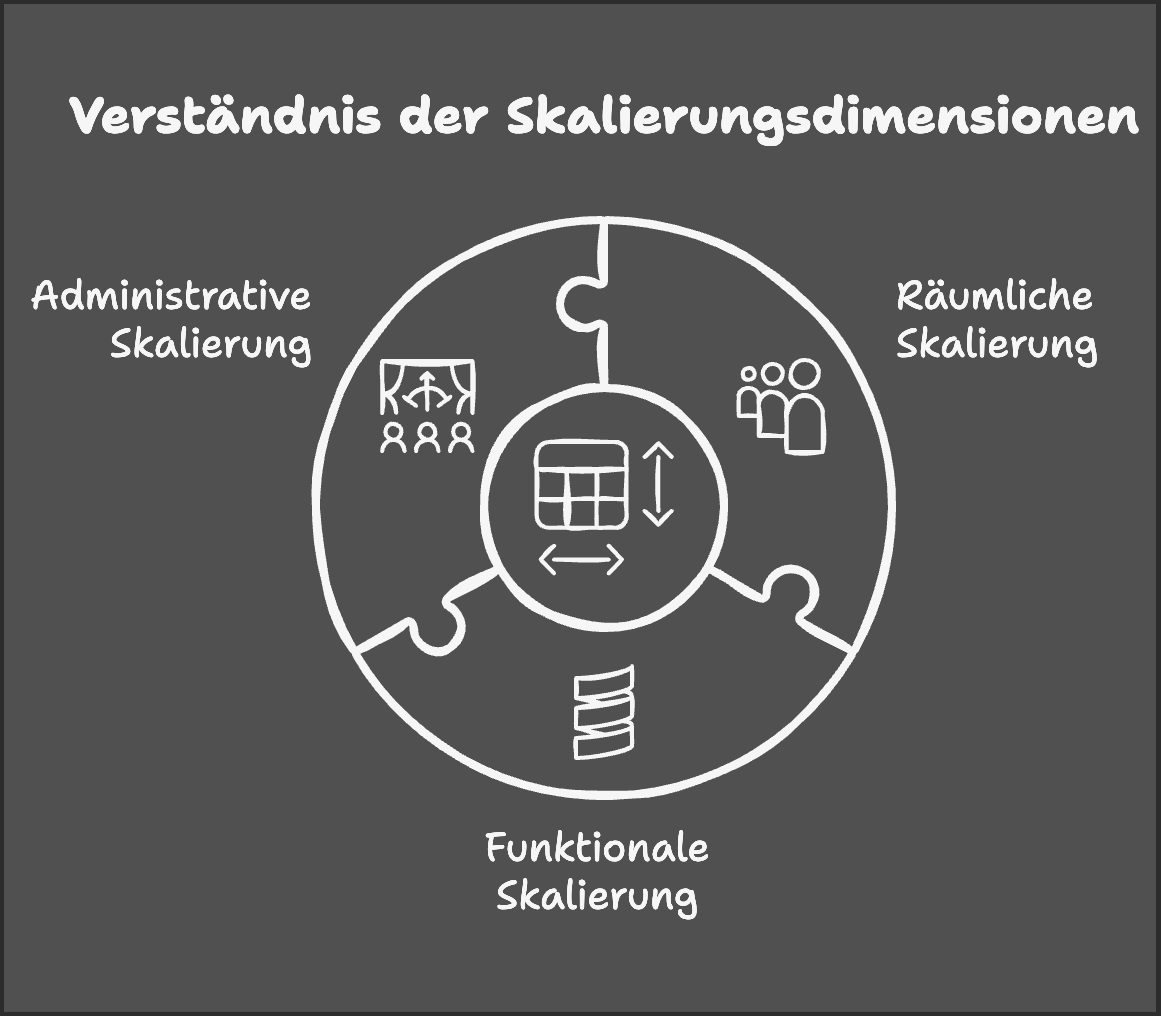
\includegraphics[width=0.8\textwidth]{fig/Skalierung.png}
           
                \caption{Symbolbild Skalierung}
            \end{figure}
        \end{column}

    \end{columns}
\end{frame}

\begin{frame}{Weiter funktionale Skalierbarkeit}
    Vielleicht aus DB zwei Ansätze für Archtiektur von functionalen Systemen:
    \begin{itemize}
    \item \textbf{vertikale Skalierung}
    \item \textbf{horizontale Skalierung}
    \end{itemize}
\end{frame}

\begin{frame}{Grenzen der Skalierbarkeit -- Little's Law}
    \textbf{Little's Law} besagt: Die durchschnittliche Anzahl an Kunden in einem System ist gleich der Ankunftsrate multipliziert mit der durchschnittlichen Verweilzeit der Kunden im System.  
    \mbox{}\\    \mbox{}\\
    Dies impliziert, dass die Skalierbarkeit eines Systems begrenzt ist durch die Fähigkeit, Anfragen zu verarbeiten, und dass eine zunehmende Anfragerate zu längeren Wartezeiten führen kann.  Stellen Sie sich eine Warteschlange in einem Supermarkt vor: Je mehr Kunden ankommen, desto länger wird die Warteschlange.
\end{frame}



\begin{frame}{Grenzen der Skalierbarkeit -- Gustafson's Law}
\textbf{Gustafson's Law} besagt: Die Problemgröße kann mit einer Erhöhung der Anzahl von Prozessoren erhöht werden, während die Zeit zur Lösung des Problems relativ konstant bleibt. 
\mbox{}\\    \mbox{}\\
Dies impliziert, dass die Parallelisierung ein Schlüssel zur Skalierbarkeit ist.  Denken Sie an ein Team von Bauarbeitern:  Je mehr Arbeiter, desto größer das Haus, das sie in der gleichen Zeit bauen können.
\end{frame}

\begin{frame}{Grenzen der Skalierbarkeit -- Amdahl's Law}
    \textbf{Amdahl's Law} besagt:  Die maximale Beschleunigung durch Parallelisierung ist begrenzt durch den Anteil der Berechnung, der nicht parallelisiert werden kann.  
    \mbox{}\\     \mbox{}\\
    Dies impliziert, dass die nicht parallelisierbaren Anteile minimiert werden sollten, um eine optimale Leistungssteigerung zu erzielen.  Stellen Sie sich eine Straße mit einem einspurigen Abschnitt vor:  Egal wie viele Spuren die Straße sonst hat, der einspurige Abschnitt begrenzt den Verkehrsfluss.

\end{frame}

\begin{frame}{Grenzen der Skalierbarkeit -- Brooks' Law}
 \textbf{Brooks' Law} besagt: Durch Hinzufügen von Ressourcen kann die Komplexität eines Systems nicht reduziert werden.  Im Gegenteil, es kann sogar zu mehr Komplexität und Overhead führen.  
 \mbox{}\\    \mbox{}\\
 Stellen Sie sich ein Softwareprojekt vor: Je mehr Entwickler beteiligt sind, desto komplexer wird die Kommunikation und Koordination.
\end{frame}

\begin{frame}{Gruppenarbeit: Gesetze}
      \begin{itemize}
        \item Handout:  2A-Skalierbarkeitsgesetze-Handout.pdf
        \item Aufgaben: 2A-Skalierbarkeitsgesetze-Aufgaben.pdf    
      \end{itemize}
\end{frame}


\begin{frame}{Verteilungstransparenz im Detail}

Komplexität des verteilten Systems vor dem Benutzer zu verbergen:

    \begin{itemize}
        \item \textbf{Zugriffstransparenz:}  Ort und Art des Zugriffs auf Ressourcen sind verborgen.
        \item \textbf{Ortstransparenz:} Der physische Speicherort der Ressourcen ist verborgen.
        \item \textbf{Migrationstransparenz:}  Ressourcen können verschoben werden, ohne dass der Benutzer es merkt.
        \item \textbf{Replikationstransparenz:}  Die Existenz von Replikaten ist verborgen.
        \item \textbf{Fehlertransparenz:}  Fehler werden vom Benutzer verborgen.
        \item \textbf{Nebenläufigkeitstransparenz:} Parallele Zugriffe auf Ressourcen sind verborgen.
        \item \textbf{Persistenztransparenz: }  Zustand eines Prozesses oder einer Anwendung bleibt unabhängig von Unterbrechungen erhalte (
    \end{itemize}
    Hinweis 1: Persistenztransparenz und Relocation immer häufiger\mbox{}\\
    Hinweis 2: Vielleicht Störungsgefühl da aus Sicht des Nutzers. \mbox{}\\
\end{frame}


\begin{frame}{Kohärenz}
  Ein verteiltes System verhält sich kohärent, wenn es sich für den Benutzer so verhält, als würden alle Daten und Funktionen an einem zentralen Ort bereitgestellt, obwohl sie tatsächlich auf verschiedene Knoten im System verteilt sind. 
  \mbox{}\\
  Das Ziel ist, die Komplexität des verteilten Systems zu verbergen und eine einheitliche und konsistente Benutzererfahrung zu bieten.
\end{frame}



\begin{frame}{Ziele im Anforderungsprozess}
    Im Anforderungsprozess für verteilte Systeme müssen die Ziele und Anforderungen klar definiert werden, um sicherzustellen, dass das System die beabsichtigten Ergebnisse liefert.  Dazu gehört die Berücksichtigung von Aspekten wie Funktionalität, Leistung, Skalierbarkeit, Sicherheit, Wartbarkeit, Portabilität, Benutzerfreundlichkeit, Anpassbarkeit und Kompatibilität.  Jeder dieser Aspekte kann je nach den spezifischen Anforderungen des Systems unterschiedlich gewichtet werden.
\end{frame}



\begin{frame}{Herausforderungen - The Eight Fallacies of Distributed Computing (1/2)}
  Diese "Fehlschlüsse" verdeutlichen häufige, aber falsche Annahmen über verteilte Systeme:
  \begin{itemize}
    \item Das Netzwerk ist immer verfügbar.
    \item Die Latenzzeit ist 0.
    \item Die Bandbreite ist unbegrenzt.
    \item Das Netzwerk ist sicher.
  \end{itemize}
  Diese Annahmen können zu schwerwiegenden Problemen führen, wenn sie bei der Entwicklung und Bereitstellung von verteilten Systemen nicht berücksichtigt werden.
\end{frame}


\begin{frame}{Herausforderungen - The Eight Fallacies of Distributed Computing (2/2)}
  Fortsetzung der "Fehlschlüsse":
  \begin{itemize}
    \item Die Topologie ändert sich nicht.
    \item Es gibt nur einen Administrator.
    \item Die Transportkosten sind null.
    \item Das Netzwerk ist homogen.
  \end{itemize}
  Die Berücksichtigung dieser Fehlschlüsse ist entscheidend für den Entwurf robuster und zuverlässiger verteilter Systeme.
\end{frame}

\begin{frame}{Diskussion: Neue Sicht auf Fehler}

  \begin{itemize}
    \item Fehler ist keine Ausnahme, sondern die Regel!
    \item Aufbau Incident Management
    \item Teststrategien hilfreich 
  \end{itemize}
\end{frame}

\end{document}